\documentclass[main.tex]{subfiles}
\begin{document}

\section{Electron scattering}

\subsection{Compton scattering onto an electron at rest}

\marginpar{Sunday\\ 2020-8-23, \\ compiled \\ \today}

We need to account for the fact that light has a quantum nature, which is not addressed in the classical treatment of scattering. 
Also, now we will account for the momentum of the photon. 

We start of with an electron at rest, and a photon with energy \(h \nu \) and momentum \(h \nu / c\) impinging on it. 
After the scattering, the photon will have energy \(h \nu '\) and momentum \(h \nu ' / c\), while the electron will have momentum \(m v \gamma \). 
Let us call the angle between the direction of the incoming photon and the direction of the outgoing one \(\theta \). 

In terms of four-vectors, we can express the momenta of the photon before and after as 
%
\begin{align}
k^{\mu } = \frac{\epsilon}{c} \left[\begin{array}{c}
1 \\ 
\vec{\Omega}
\end{array}\right]
\qquad \text{and} \qquad
k^{\prime \mu } = \frac{\epsilon'}{c} \left[\begin{array}{c}
1 \\ 
\vec{\Omega}'
\end{array}\right]
\,,
\end{align}
%
where \(\vec{\Omega}\) and \(\vec{\Omega}'\) are unit vectors defining the propagation directions, such that \(\vec{\Omega} \cdot \vec{\Omega}' = \cos \theta \). 
On the other hand, the momenta of the electron will be 
%
\begin{align}
p^{\mu }  = \left[\begin{array}{c}
mc \\ 
\vec{0}
\end{array}\right]
\qquad \text{and} \qquad
p^{\prime \mu } = \gamma \left[\begin{array}{c}
mc \\ 
m \vec{v}
\end{array}\right]
\,.
\end{align}

Since the particles are unchanged after the scattering, both the incoming and outgoing momenta must satisfy \(p^{\mu } p_{\mu } = - m^2 c^2\) and \(k^{\mu } k_{\mu } = 0\) (in any frame: they are Lorentz scalars). 
Because of momentum conservation, we can also impose the four equations 
%
\begin{align}
p^{\mu } + k^{\mu } = p^{\prime \mu } + k^{\prime \mu }
\,.
\end{align}

Solving the system of equations yields 
%
\begin{align}
\epsilon' = \frac{\epsilon }{1 + \frac{\epsilon }{mc^2} \qty(1 - \vec{\Omega} \cdot \vec{\Omega}')}
\,,
\end{align}
%
implying that we must have \(\epsilon' \leq \epsilon \): the photon will lose energy in the scattering. 
The calculation which yields the differential cross section of the scattering is quite complicated and requires the full machinery of QED; here we just give the result: 
%
\begin{align}
\frac{ \dd{\sigma }  }{ \dd{\vec{\Omega} }'} 
= \frac{r_0^2}{2 } \qty(\frac{\epsilon '}{\epsilon })^2
\qty[ \frac{\epsilon}{\epsilon '} + \frac{\epsilon'}{\epsilon } - (1 - \vec{\Omega} \cdot \vec{\Omega}')^2] 
\,,
\end{align}
%
where \(\epsilon \) is the energy divided by \(m c^2\) and \(r_0 \) is the classical electron radius. 
\todo[inline]{Missing square for the \(\sin \theta \) term in the KN cross section! see \cite[eq.\ 7.4]{rybickiRadiativeProcessesAstrophysics1979}.}

If we substitute in our formula for the energy, using \(\xi = \cos \theta = \vec{\Omega} \cdot \vec{\Omega}'\), we find 
%
\begin{align}
\frac{ \dd{\sigma }}{ \dd{\Omega }' \dd{\epsilon }'} 
= \frac{r_0^2}{2} \frac{1 + \xi^2}{\qty(1 + \epsilon (1 - \xi ))^2}
\qty[1 + \frac{\epsilon^2 (1 - \xi )^2}{(1 + \xi )^2 (1 + \epsilon (1 - \xi ))}]
\delta \qty(\epsilon ' - \frac{\epsilon }{1 + \epsilon (1 - \xi )})
\,.
\end{align}

We have inserted a \(\dd{\epsilon '}\) differential for the outgoing photon energy, we are considering a density in one more variable but it is singular there, whence the \(\delta \) function, which describes the distribution in \(\epsilon '\) space --- concentrated at the only value allowed by 4-momentum conservation. 
Note that this makes sense dimensionally, as the dimension of a \(\delta \) function is the inverse of the dimension of its argument. 

In the low energy limit, \(h \nu \ll m_e c^2 \) or \(\epsilon \to 0\), we find 
%
\begin{align}
\frac{ \dd{\sigma }}{ \dd{\Omega }' \dd{\epsilon }'} 
=
\frac{r_0^2}{2} (1 + \xi^2) \delta (\epsilon ' - \epsilon )
\,,
\end{align}
%
which is the Thomson cross section. 

Let us now define the \textbf{Compton scattering kernel} \(\sigma \): it is the differential cross section times the electron density,
%
\begin{align}
\sigma (\epsilon \to \epsilon ', \xi ) = n_e \frac{ \dd{\sigma }}{ \dd{\Omega }' \dd{\epsilon }'}
\,.
\end{align}

We can integrate this in order to find the total cross section presented by the electrons to photons of an energy \(\epsilon \): 
%
\begin{align}
\sigma (\epsilon ) &= \int \dd{\Omega '} \dd{\epsilon '} \sigma (\epsilon \to \epsilon ', \xi ) \\
&= \frac{3}{4} n_e \sigma_{T} \qty[ \qty(\frac{1 + \epsilon }{\epsilon^3}) 
\qty(\frac{2 \epsilon (1 + \epsilon )}{1 + 2 \epsilon }- \log \qty(1 + 2 \epsilon ))
+ 
\frac{1}{2 \epsilon } \log \qty(1 + 2 \epsilon )
- 
\frac{1 + 3 \epsilon }{(1 + 2 \epsilon )^2}
]
\,.
\end{align}

How does this differ from the Thomson cross section? For \(\log \epsilon \lesssim -1 \) we have \(\sigma \approx \sigma_T\), while as \(\epsilon \) increases the cross section goes to zero. 

\begin{figure}[ht]
\centering
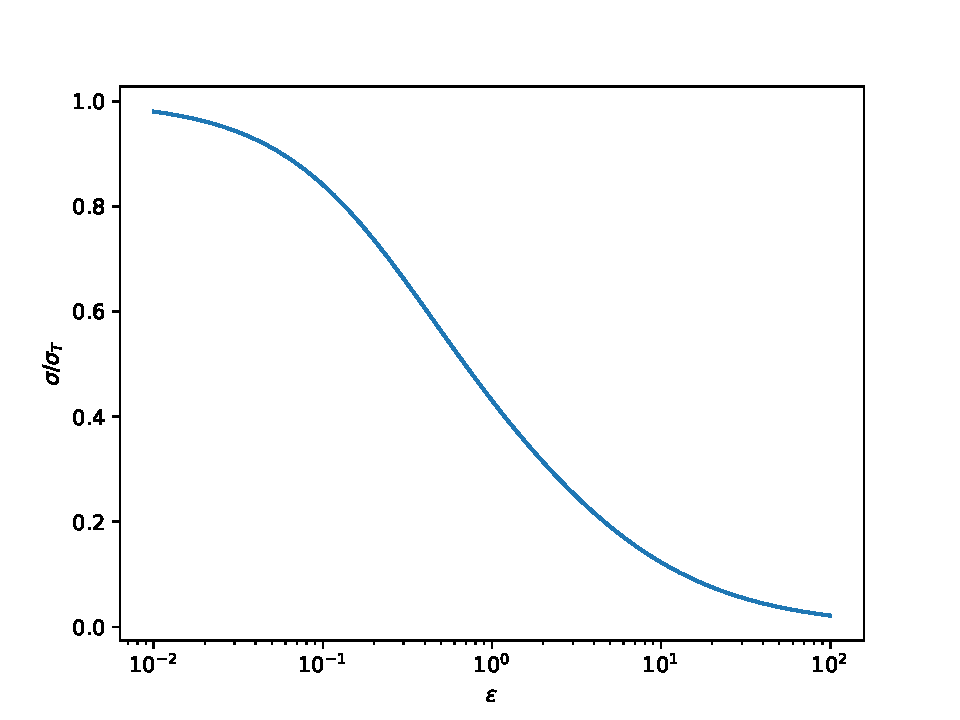
\includegraphics[width=\textwidth]{figures/compton-sigma.pdf}
\caption{Compton cross section as a function of \(\epsilon \), photon energy by \(m_e c^2\). }
\label{fig:compton-sigma}
\end{figure}

In the low energy limit we have the expansion 
%
\begin{align}
\sigma (\epsilon )\approx \sigma_T \qty(1 -2 \epsilon + \frac{26}{5} \epsilon^2)
\,.
\end{align}

The introduction of these nonconservative aspects complicates the radiative transfer equation for scattering.
The absorption term is 
%
\begin{align}
- \alpha _\nu ^{(s)} I _\nu =  
- I (\epsilon , \Omega ) n_e \int \dd{\Omega }' \dd{\epsilon }' \frac{ \dd{\sigma }}{ \dd{\Omega }' \dd{\epsilon }' } =     - I (\epsilon , \Omega  ) \sigma (\epsilon )
\,,
\end{align}
%
while for the emission term the intensity must go inside the integral, so we have 
%
\begin{align}
j_\nu^{(s)} = 
n_e \int \dd{\Omega }' \dd{\epsilon '} I(\epsilon ', \Omega ') \frac{ \dd{\sigma }}{ \dd{\Omega }' \dd{\epsilon }' } = \int \dd{\Omega }' \dd{\epsilon }'
I(\epsilon ', \Omega ')
 \sigma (\epsilon \to \epsilon ', \xi )
\,,
\end{align}
%
which cannot be expressed in terms of the integrated kernel \(\sigma (\epsilon )\). 

For Thomson scattering the absorption term is similar, with \(n_e \sigma_T\) instead of \(\sigma (\epsilon )\). 
The emission term, on the other hand, can now be evaluated to yield  
%
\begin{align}
\int \dd{\Omega }' \dd{\epsilon }' \sigma (\epsilon \to \epsilon ', \xi )
= \frac{r_0^2}{2} n_e \int \dd{\Omega '} \dd{\epsilon '} I(\epsilon ', \Omega ') (1 + \xi^2) \delta (\epsilon ' - \epsilon ) \sim n_e \sigma_T J(\epsilon )
\,,
\end{align}
%
as long as we neglect the angular dependence of the intensity. 

We are always restricting ourselves to electrons which are initially at rest. For them Thomson scattering is a good approximation; photons more energetic than a few tens of \SI{}{keV} (hard X-rays) hardly scatter, since the Klein-Nishina cross section drops at high energies.

So, by using the Thomson limit we do not get it wrong by much. 

The main conclusions we can draw from this is that we expect no spectral modifications (since Thomson scattering is conservative) but we do expect angular redistribution (since Thomson scattering is essentially isotropic).

\subsection{Scattering in plasmas}

Electrons are not at rest in any realistic astrophysical setting. In order to have free electrons we need a plasma, which is made of (at least partially) ionized gas. 
So, we need a way to describe the fractional ionization.
Let us consider only hydrogen for simplicity: we define the collisional ionization fraction \(x\) (ionized atoms divided by total atoms), which can be expressed in terms of the temperature as 
%
\begin{align}
x = \frac{F}{1 + F} 
\qquad \text{where} \qquad
F = 2T \exp(-\frac{\SI{1.58e5}{K}}{T})
\,.
\end{align}

The way \(x\) looks as a function of temperature is a kind of sigmoid: it is close to zero, then at \(T\) around \SI{e4}{K} it quickly rises, and becomes close to 1 at a few times \SI{e4}{K}. At temperatures larger than \SI{e5}{K} the plasma is basically fully ionized (which makes sense: the first ionization energy of hydrogen is \(\SI{13.6}{eV} \approx \SI{1.6e5}{K}\)). 

At these temperatures, the electrons will be moving quite a lot because of thermal motion. 

\subsection{Inverse Compton scattering}

Scattering onto moving electrons is often called \textbf{inverse Compton scattering}, since in this case the photon might gain energy instead of losing it. 
We start off with a photon with momentum \(k^{\mu } = (\epsilon /c) (1, \vec{\Omega})\) and an electron with momentum \(p^{\mu } = \gamma (mc, m \vec{v})\); the outgoing electron and momentum momenta, energies and velocities will be denoted with a prime. 

We know how to deal with scattering off a stationary electron, and stationarity is relative: if we boost to the electron's rest frame we can apply the results from regular Compton scattering, and then we will need to boost back to our frame. 

We shall denote quantities calculated in the ERF (electron rest frame) with a pedix \(e\): for example the energy of the photon in the ERF before the scattering will be \(\epsilon_e\).
This means that in the ERF we will have the equality 
%
\begin{align}
\epsilon_e' 
= \frac{\epsilon_e}{1 + \frac{\epsilon_e}{mc^2} (1 - \cos \Theta )} 
\approx \epsilon_e \qty(1 - \frac{\epsilon_e}{mc^2} (1 - \cos \Theta )) 
\approx \epsilon_e 
\qquad \text{if } \epsilon_e \ll m c^2 
\,.
\end{align}

We are saying that in the rest frame the scattering will basically be conservative, this is for sure an approximation but, because of what we discussed earlier about the Klein-Nishina cross section dropping off at high energies, not a large one. 

The Lorentz transform from the LAB frame to the ERF for the energy of the photon is: 
%
\begin{align}
\epsilon_e = \gamma \epsilon \qty(1 - \beta \cos \theta )
\,,
\end{align}
%
while the transform back from  the ERF to the LAB frame is 
%
\begin{align}
\epsilon' = \gamma \epsilon_e' \qty(1 + \beta \cos \theta _e )
\,.
\end{align}

Note that the quantities \(\beta \) and \(\gamma \) refer to the velocity of the electron: since we are approximating the scattering as conservative in the ERF calculating them before or after the scattering is the same (the direction of the electron can change: this is accounted for by letting \(\theta\) and \(\theta '\) be different). 
So, we can just insert these two multiplicative factors one after another to find the total change in energy of the photon: 
%
\begin{align}
\epsilon ' &\approx \gamma^2 \epsilon \qty(1 - \beta \cos \theta ) \qty(1 + \beta \cos \theta'_e ) 
\,.
\end{align}

\todo[inline]{Inaccuracy in the slides: the first formula does not really make sense, since the approximation of the nonconservativeness factor being equal to one has been made in part of it (\(\beta \) and \(\gamma \) being the same before and after), so it does not make sense to write it out.}

Let us neglect the angular terms for now: generally they are of order unity. Instead, the main factor in the formula is \(\gamma^2>1\): this means that in general the energy of the scattered photon is of the order \(\epsilon ' = \gamma^2 \epsilon > \epsilon  \). 
The boost of the energy of the photon depends on how relativistic the electron is; if the electron is very relativistic the boost in energy for the photon can be quite large. 

In order to make predictions about the effect of this for a population of electrons and photons, we can Lorentz transform the Compton Scattering Kernel: the final result of the manipulation is
%
\begin{align}
\sigma (\epsilon \to \epsilon ', \xi ) = \frac{D}{D'} \sigma_e \qty(\epsilon _e \to \epsilon _e', \xi _e)
\,,
\end{align}
%
where \(D = 1 - \vec{\Omega} \cdot \vec{v} / c = 1 - \beta \cos \theta \) and \(D' = 1 - \vec{\Omega}' \cdot \vec{v}' / c \approx 1 + \beta \cos \theta '_e\) are the factors in the Lorentz transforms, which allow us to write \(\epsilon _e = \gamma D \epsilon \) and \(\epsilon _e' = \gamma D' \epsilon '\).

The transformation law for \(\xi = \vec{\Omega} \cdot \vec{\Omega}\) is 
%
\begin{align}
1 - \xi = \frac{1 - \xi _e}{\gamma^2 D D'}
\,,
\end{align}
%
while the electron energy density transforms as \(n = \gamma n_e\). 

This allows us to write down an explicit expression for \(\sigma (\epsilon \to \epsilon ', \vec{\Omega}, \vec{\Omega}')\) in the lab frame for a population of single-speed electrons:
%
\begin{align}
\sigma (\epsilon \to \epsilon ', \vec{\Omega}, \vec{\Omega}', v) 
= 
\frac{n r_0^2}{2 \epsilon \nu \gamma } 
\qty[1 + \qty(1 + \frac{1 - \xi }{\gamma^2 D D'})^2
+ \frac{\epsilon \epsilon ' (1 - \xi )^2}{\gamma^2 D D'}]
\delta \qty(\xi -1 + \frac{\gamma D}{\epsilon'} - \frac{\gamma D'}{\epsilon })
\,,
\end{align}
%
but we must also consider the fact that the electrons are distributed with different velocities: if their distribution is isotropic, so that \(\dd{n} = n f(v) \dd[3]{v}\) then we can integrate across all velocity space, getting an expression like 
%
\begin{align}
\sigma (\epsilon \to \epsilon ', \xi )
= \int \dd{v} \sin \theta_v \dd{\theta _v} \dd{\phi _v}
 v^2 n f(v) 
\sigma (\epsilon \to \epsilon ', \vec{\Omega}, \vec{\Omega}', v)  
\,.
\end{align}



\end{document}
